\section{Model}
\label{sec:model}

\setlength{\tabcolsep}{2pt}
\begin{figure*}
\begin{center}
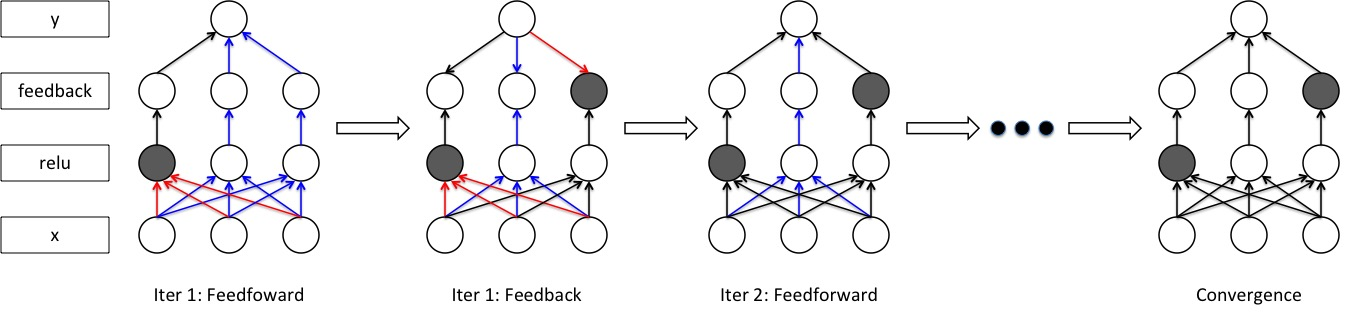
\includegraphics[width=0.95\linewidth]{figs/model/model}
% \vspace{-10pt}
\caption{Illustration of our feedback model and its inference process. At the first iteration, the model performs as a feedforward neural net. Then given the top signal neuron, the hidden layers update their gates to maximize the confidence for the top neuron. This process continues until convergence.}
\label{fig:visual_compare}
% \vspace{-30pt}
\end{center}
\end{figure*}

\subsection{Convolutional Neural Networks}

\subsection{Infering the Hidden Neurons, the Discriminative Framework}
%In deformable part based model, the joint probability P(y, h, x, \theta). Given an image x, a model \theta and label y, we want to infer the hidden neurons for a better understanding and fit to the images given the label.

% P(y, h | x, \theta) \propto P(y | h, x, \theta) P(h | x, \theta)

We model the top down as another type of activation variable, similar as ReLu. However, this unit activates based on the the overall information of bottom-up responses and top-down messages. 

In practice, we treat the inference process as discriminatively optimize the final class node. 

%max_h f(y | h, x, \theta)

Optimizing such function results in an integer programming, if we treat h as binary variables. 

During optimization, we proposed two ways to deal with it, 1. coordinate descent 2. continuous relaxation

Hard optimization: The coordinate descent frameworks stand in this way: 1. Initialize h as all 1 meaning the gate is open, compute feedfoward messages to the class node, then given the current activation status, optimize the last layer h to maximize the class output, given the updates last layer h, keep optimizing lower layers. And reiterate this process.

Soft optimization: The continuous relaxation falls in below way, compute the gradient of class node y given h, use gradient descent update h, and keep until this until convergence.

\subsection{Class Model Visualization}

Following this, deconvnet can be viewed as a one iteration of our hard optimization

\textbf{Relationship to Oxford and Deconv}

\subsection{Object Localization}

In this section we describe how a classification ConvNet can be queried about the spatial support of a particular class in a given image. Given an image I0, a class c, and a classification ConvNet with the class score function Sc(I), we would like to rank the pixels of I0 based on their influence on the score Sc(I0). 
We start with a motivational example. Consider the linear score model for the class c: 
%Sc(I) = wcT I + bc, (2) 
where the image I is represented in the vectorised (one-dimensional) form, and wc and bc are respectively the weight vector and the bias of the model. In this case, it is easy to see that the magnitude of elements of w defines the importance of the corresponding pixels of I for the class c. 
In the case of deep ConvNets, the class score Sc(I) is a highly non-linear function of I, so the reasoning of the previous paragraph can not be immediately applied. However, given an image I0, we can approximate Sc(I) with a linear function in the neighbourhood of I0 by computing the first-order Taylor expansion: 
%Sc(I) ≈ wT I + b, (3) where w is the derivative of Sc with respect to the image I at the point (image) I0: 
%w=∂Sc􏰁􏰁􏰁 . (4) ∂I 􏰁I0 
Another interpretation of computing the image-specific class saliency using the class score deriva- tive (4) is that the magnitude of the derivative indicates which pixels need to be changed the least to affect the class score the most. One can expect that such pixels correspond to the object location in the image. We note that a similar technique has been previously applied by [1] in the context of Bayesian classification. 

Given an image I0 (with m rows and n columns) and a class c, the class saliency map M ∈ Rm×n is computed as follows. First, the derivative w (4) is found by back-propagation. After that, the saliency map is obtained by rearranging the elements of the vector w. In the case of a grey-scale image, the number of elements in w is equal to the number of pixels in I0, so the map can be computed as Mij = |wh(i,j)|, where h(i, j) is the index of the element of w, corresponding to the image pixel in the i-th row and j-th column. In the case of the multi-channel (e.g. RGB) image, let us assume that the colour channel c of the pixel (i, j) of image I corresponds to the element of w with the index h(i,j,c). To derive a single class saliency value for each pixel (i,j), we took the maximum magnitude of w across all colour channels: Mij = maxc |wh(i,j,c)|. 
It is important to note that the saliency maps are extracted using a classification ConvNet trained on the image labels, so no additional annotation is required (such as object bounding boxes or segmentation masks). The computation of the image-specific saliency map for a single class is extremely quick, since it only requires a single back-propagation pass. 
We visualise the saliency maps for the highest-scoring class (top-1 class prediction) on randomly se- lected ILSVRC-2013 test set images in Fig. 2. Similarly to the ConvNet classification procedure [8], where the class predictions are computed on 10 cropped and reflected sub-images, we computed 10 saliency maps on the 10 sub-images, and then averaged them. 
The weakly supervised class saliency maps (Sect. 3.1) encode the location of the object of the given class in the given image, and thus can be used for object localisation (in spite of being trained on image labels only). Here we briefly describe a simple object localisation procedure, which we used for the localisation task of the ILSVRC-2013 challenge [12]. 
Given an image and the corresponding class saliency map, we compute the object segmentation mask using the GraphCut colour segmentation [3]. The use of the colour segmentation is motivated by the fact that the saliency map might capture only the most discriminative part of an object, so saliency thresholding might not be able to highlight the whole object. Therefore, it is important to be able to propagate the thresholded map to other parts of the object, which we aim to achieve here using the colour continuity cues. Foreground and background colour models were set to be the Gaussian Mixture Models. The foreground model was estimated from the pixels with the saliency higher than a threshold, set to the 95% quantile of the saliency distribution in the image; the background model was estimated from the pixels with the saliency smaller than the 30% quantile (Fig. 3, right-middle). The GraphCut segmentation [3] was then performed using the publicly available implementation2. Once the image pixel labelling into foreground and background is computed, the object segmentation mask is set to the largest connected component of the foreground pixels (Fig. 3, right). 
We entered our object localisation method into the ILSVRC-2013 localisation challenge. Consid- ering that the challenge requires the object bounding boxes to be reported, we computed them as the bounding boxes of the object segmentation masks. The procedure was repeated for each of the top-5 predicted classes. The method achieved 46.4% top-5 error on the test set of ILSVRC-2013. It should be noted that the method is weakly supervised (unlike the challenge winner with 29.9% error), and the object localisation task was not taken into account during training. In spite of its simplicity, the method still outperformed our submission to ILSVRC-2012 challenge (which used the same dataset), which achieved 50.0% localisation error using a fully-supervised algorithm based on the part-based models [6] and Fisher vector feature encoding [11]. 

\textbf{Relationship to Oxford and Deconv}
